\cmfnewsection{Visão Geral do PSCAD e do Curso}{./logos/fundo_tese}{0.15}






%%%%%%%%%%%%%%%%%%%%%%%%%%%%%%%%%%%%%%%%%%%%%%%%
%%%%%%%%%%%%%%%%%%%%%%%%%%%%%%%%%%%%%%%%%%%%%%%%
%%%%%%%%%%%%%%%%%%%%%%%%%%%%%%%%%%%%%%%%%%%%%%%%
%%%%%%%%%%%%%%%%%%%%%%%%%%%%%%%%%%%%%%%%%%%%%%%%
\begin{frame}{Objetivo}
\centering

\begin{itemize}
\item Aprender a montar simulações de sistemas elétricos no PSCAD 
\vspace*{1cm}
\item Aprender a extrair resultados
\vspace*{1cm}
\item Possivelmente, aprender o funcionamento de alguns circuitos básicos.
\vspace*{1cm}
\end{itemize}

\end{frame}






%%%%%%%%%%%%%%%%%%%%%%%%%%%%%%%%%%%%%%%%%%%%%%%%
%%%%%%%%%%%%%%%%%%%%%%%%%%%%%%%%%%%%%%%%%%%%%%%%
%%%%%%%%%%%%%%%%%%%%%%%%%%%%%%%%%%%%%%%%%%%%%%%%
%%%%%%%%%%%%%%%%%%%%%%%%%%%%%%%%%%%%%%%%%%%%%%%%
\begin{frame}{O que é o PSCAD}
\centering

\begin{itemize}
\item O PSCAD ({\it Power Systems Computer Aided Design}) é uma interface gráfica para simulação no EMTDC

\vspace*{2cm}

\item o EMTDC é um programa utilizado para simulação de transitórios eletromagnéticos.
\end{itemize}

\end{frame}





%%%%%%%%%%%%%%%%%%%%%%%%%%%%%%%%%%%%%%%%%%%%%%%%
%%%%%%%%%%%%%%%%%%%%%%%%%%%%%%%%%%%%%%%%%%%%%%%%
%%%%%%%%%%%%%%%%%%%%%%%%%%%%%%%%%%%%%%%%%%%%%%%%
%%%%%%%%%%%%%%%%%%%%%%%%%%%%%%%%%%%%%%%%%%%%%%%%
\begin{frame}{Para que serve o PSCAD}
\centering

\begin{itemize}
\item Simulação de sistemas de potência: transitórios eletromagnéticos

\begin{itemize}
\item Redes de distribuição e transmissão
\item Máquinas Elétricas
\item Sistemas de controle de fontes de energia
\end{itemize}

\vspace*{1cm}

\item Simulação de sistemas envolvendo eletrônica de potência.

\begin{itemize}
\item Grid-connected/Grid-Forming Converters
\item HVDCs ({\it High Voltage Direct Current})
\item FACTS ({\it flexible alternating current transmission system})
\item Sistemas de controle
\end{itemize}

\end{itemize}

\end{frame}





%%%%%%%%%%%%%%%%%%%%%%%%%%%%%%%%%%%%%%%%%%%%%%%%
%%%%%%%%%%%%%%%%%%%%%%%%%%%%%%%%%%%%%%%%%%%%%%%%
%%%%%%%%%%%%%%%%%%%%%%%%%%%%%%%%%%%%%%%%%%%%%%%%
%%%%%%%%%%%%%%%%%%%%%%%%%%%%%%%%%%%%%%%%%%%%%%%%
\begin{frame}{Ideia Geral do PSCAD}
\centering


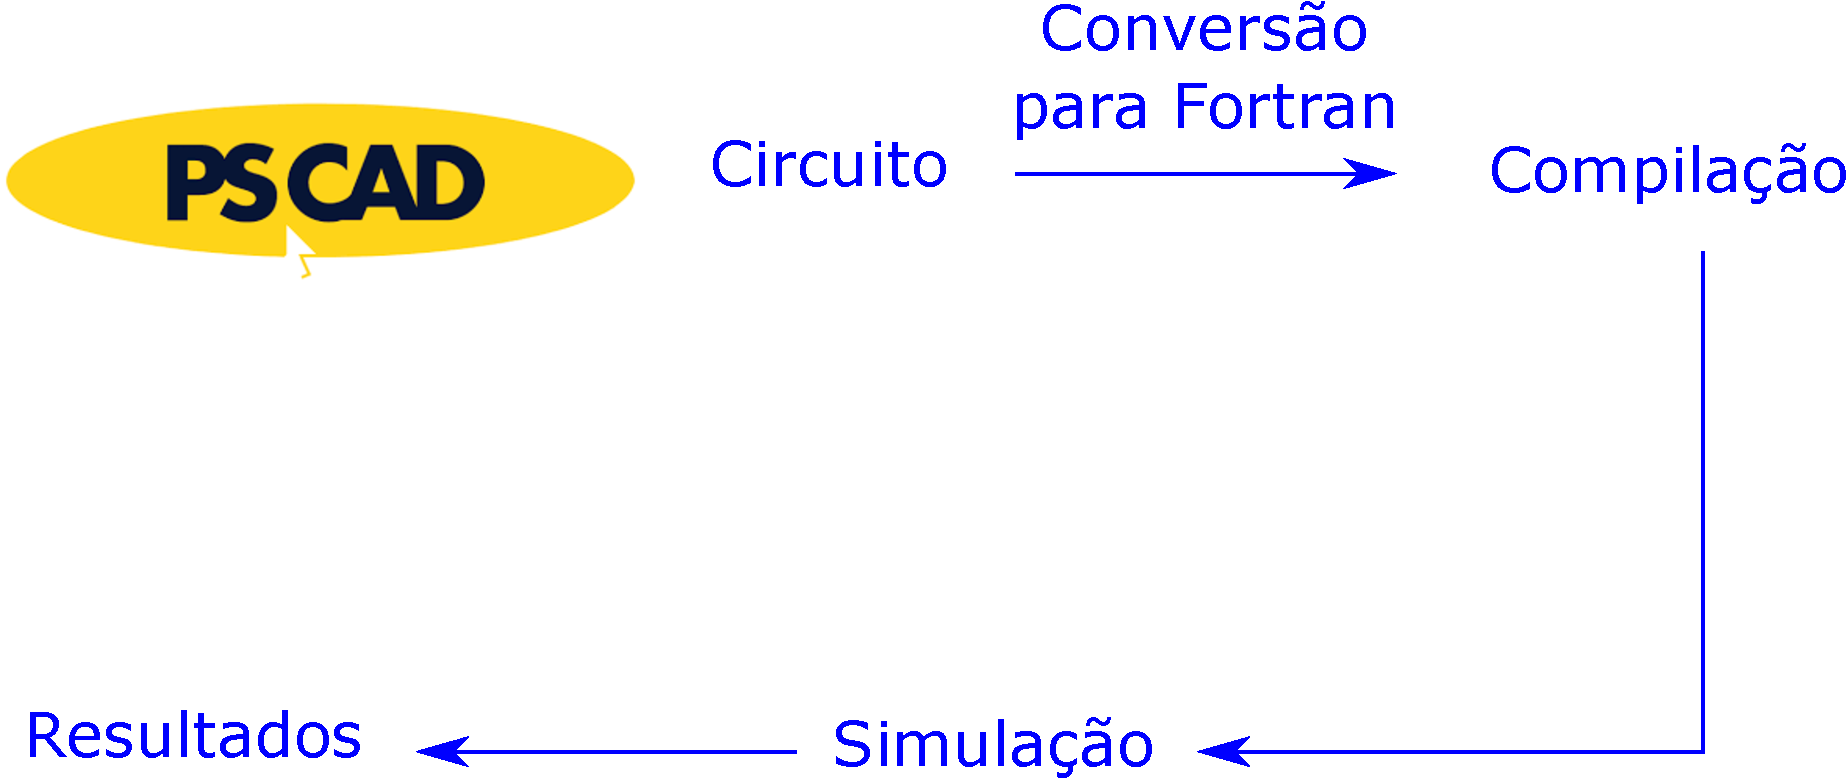
\includegraphics[width=0.95\linewidth]{./figuras/geral/fluxo}

\end{frame}
